\documentclass[11pt,a4paper]{article}
\usepackage[margin=2.2cm]{geometry}
\usepackage{lmodern}
\usepackage[T1]{fontenc}
\usepackage{microtype}
\usepackage{amsmath,amssymb,amsthm,bm,mathtools}
\usepackage{booktabs,array}
\usepackage{graphicx}
\usepackage[dvipsnames]{xcolor}
\usepackage[most]{tcolorbox}
\usepackage{enumitem}
\usepackage[colorlinks=true,linkcolor=MidnightBlue,urlcolor=MidnightBlue]{hyperref}
\setlength{\parskip}{4pt}\setlength{\parindent}{0pt}
\setlist{itemsep=2pt,topsep=3pt}

\newtcolorbox{plainbox}{colback=blue!4,colframe=MidnightBlue,title=In plain words,fonttitle=\bfseries\small,boxrule=0.6pt,arc=2pt,breakable}
\newtcolorbox{watchbox}{colback=orange!6,colframe=BurntOrange,title=Watch out,fonttitle=\bfseries\small,boxrule=0.6pt,arc=2pt,breakable}
\newtcolorbox{oursbox}{colback=green!5,colframe=ForestGreen,title=What we do in our 2D version,fonttitle=\bfseries\small,boxrule=0.6pt,arc=2pt,breakable}
\newtcolorbox{examplebox}{colback=gray!6,colframe=gray!60,title=Worked example,fonttitle=\bfseries\small,boxrule=0.6pt,arc=2pt,breakable}
\newtcolorbox{whybox}{colback=violet!4,colframe=violet!60!black,title=Why it is true,fonttitle=\bfseries\small,boxrule=0.6pt,arc=2pt,breakable}
\newtcolorbox{algbox}[1][]{colback=white,colframe=black!50,title={#1},fonttitle=\bfseries\small,boxrule=0.6pt,arc=2pt,breakable}
\newtcolorbox{testbox}{colback=yellow!7,colframe=olive!70!black,title=How to check your code,fonttitle=\bfseries\small,boxrule=0.6pt,arc=2pt,breakable}

\newcommand{\vect}[1]{\mathbf{#1}}
\newcommand{\pW}{\vect{p}_W}
\newcommand{\R}{\mathbb{R}}
\newcommand{\T}{^{\top}}

\title{\textbf{The Deformable Virtual Structure, step by step}\\[3pt]
\large The mathematics of Zhou, Hou, Xu \& Gao (2025), explained from the ground up,\\
plus our extension: splitting and merging the DVS with a cell complex and a safety chain}
\date{Written for the GNSS-denied whoop swarm project, November 2026}

\begin{document}
\maketitle
\vspace{-1em}
\begin{center}
\begin{minipage}{0.9\textwidth}\small
\textbf{How to read this.} Part I collects the few mathematical tools everything else uses (vectors, polygons,
Voronoi cells, optimisation). Part II goes through the paper (arXiv:2509.18636, in \texttt{../paper/}) one idea at
a time: what it computes, \emph{why} the formula is what it is, a worked example, and what can go wrong. Part III is
our own extension: drones own cells, a DVS is a set of cells, and the DVS can split around an obstacle and merge
again, with a safety argument that holds at every step. Coloured boxes: \emph{In plain words}, \emph{Why it is true}
(short proofs), \emph{Worked example}, \emph{Watch out} (paper typos and traps), \emph{What we do in our 2D version},
and \emph{How to check your code}. No bending yet: the shape only moves, scales and squishes.
\end{minipage}
\end{center}

\tableofcontents
\newpage

%==========================================================================================
\part{Tools}
%==========================================================================================

\section{Vectors, matrices and what a matrix does to areas and distances}

We work in the plane. A point or a vector is $\vect{q}=(x,y)\T\in\R^2$. Its length is
$\|\vect{q}\|=\sqrt{x^2+y^2}$, the dot product is $\vect{a}\cdot\vect{b}=a_xb_x+a_yb_y$, and the 2D ``cross
product'' (a number) is $\vect{a}\times\vect{b}=a_xb_y-a_yb_x$. Its sign says on which side $\vect{b}$ lies: positive
means $\vect{b}$ is to the left of $\vect{a}$ (counter-clockwise turn).

A matrix $\vect{D}\in\R^{2\times2}$ maps a vector $\vect{q}$ to $\vect{D}\vect{q}$. Two facts are used again and again.

\textbf{Fact 1 (areas).} If $X$ is any region, the region $\vect{D}X=\{\vect{D}\vect{q}:\vect{q}\in X\}$ has area
\[
\operatorname{area}(\vect{D}X)=|\det\vect{D}|\cdot\operatorname{area}(X).
\]
\textbf{Fact 2 (distances).} For every vector $\vect{d}$,
\[
\sigma_{\min}(\vect{D})\,\|\vect{d}\|\ \le\ \|\vect{D}\vect{d}\|\ \le\ \sigma_{\max}(\vect{D})\,\|\vect{d}\|,
\]
where $\sigma_{\min},\sigma_{\max}$ are the smallest and largest \emph{singular values} of $\vect{D}$. For a
diagonal matrix $\mathrm{diag}(a,b)$ with $a,b>0$ they are simply $\min(a,b)$ and $\max(a,b)$.

\begin{whybox}
For $\vect{D}=\mathrm{diag}(a,b)$: $\|\vect{D}\vect{d}\|^2=a^2d_x^2+b^2d_y^2$. This lies between
$\min(a,b)^2(d_x^2+d_y^2)$ and $\max(a,b)^2(d_x^2+d_y^2)$. Take square roots. For areas: a small square of side
$\epsilon$ becomes a rectangle $a\epsilon\times b\epsilon$, so areas are multiplied by $ab=\det\vect{D}$; any region is
a union of small squares.
\end{whybox}

An \textbf{affine map} is ``matrix, then shift'': $\vect{q}\mapsto\vect{c}+\vect{D}\vect{q}$. The DVS is exactly an
affine map applied to a template shape (Section~\ref{sec:affine}). Section~\ref{sec:convaff} explains what such a map keeps and what it does not.

%------------------------------------------------------------------------------------------
\section{Polygons: area, centroid, inside test, distance to the boundary}\label{sec:polygons}

A polygon is a list of vertices $\vect{v}_0,\dots,\vect{v}_{K-1}$ in counter-clockwise (CCW) order; edge $k$ goes
from $\vect{v}_k$ to $\vect{v}_{k+1}$ (indices wrap around, $\vect{v}_K=\vect{v}_0$).

\textbf{Area (shoelace formula).}
\[
A=\frac12\sum_{k=0}^{K-1}\big(x_k\,y_{k+1}-x_{k+1}\,y_k\big)=\frac12\sum_k \vect{v}_k\times\vect{v}_{k+1}.
\]
It is positive for CCW order and negative for clockwise order, so it also tells you the orientation.

\textbf{Centroid} (centre of mass of the filled polygon, uniform density):
\[
c_x=\frac{1}{6A}\sum_k (x_k+x_{k+1})(x_ky_{k+1}-x_{k+1}y_k),\qquad
c_y=\frac{1}{6A}\sum_k (y_k+y_{k+1})(x_ky_{k+1}-x_{k+1}y_k).
\]

\begin{whybox}
Split the polygon into triangles $(\vect{0},\vect{v}_k,\vect{v}_{k+1})$. Triangle $k$ has signed area
$\tfrac12\,\vect{v}_k\times\vect{v}_{k+1}$ and centroid $(\vect{0}+\vect{v}_k+\vect{v}_{k+1})/3$. Adding the areas
gives the shoelace formula; the area-weighted average of the triangle centroids gives the centroid formula (the
factor $\tfrac12\cdot\tfrac13=\tfrac16$). Triangles that stick outside the polygon have negative area and cancel
exactly the extra parts.
\end{whybox}

\begin{examplebox}
Unit square $(0,0),(1,0),(1,1),(0,1)$. The terms $x_ky_{k+1}-x_{k+1}y_k$ are $0,1,1,0$, so $A=\tfrac12\cdot2=1$.
$c_x=\tfrac16\,[(0+1)\cdot0+(1+1)\cdot1+(1+0)\cdot1+(0+0)\cdot0]=\tfrac36=0.5$, and $c_y=0.5$ likewise.
\end{examplebox}

\textbf{Inside test, convex polygon.} $\vect{q}$ is inside (or on the boundary) iff it is on the left of every edge:
$(\vect{v}_{k+1}-\vect{v}_k)\times(\vect{q}-\vect{v}_k)\ge0$ for all $k$.
\textbf{Inside test, any polygon (ray casting).} Shoot a ray from $\vect{q}$ to the right and count edge crossings;
odd means inside.

\textbf{Distance from a point to a segment} $[\vect{a},\vect{b}]$: project and clamp,
\[
t^\star=\operatorname{clamp}\!\Big(\frac{(\vect{q}-\vect{a})\cdot(\vect{b}-\vect{a})}{\|\vect{b}-\vect{a}\|^2},\,0,\,1\Big),
\qquad d(\vect{q},[\vect{a},\vect{b}])=\big\|\vect{q}-(\vect{a}+t^\star(\vect{b}-\vect{a}))\big\|.
\]
The distance from a point to a polygon's boundary is the minimum over its edges. \textbf{Distance between two
segments}: if they cross it is $0$; otherwise it is the smallest of the four point-to-segment distances (each
endpoint to the other segment).

\textbf{Clipping a convex polygon by a half-plane} $\{\vect{q}:\vect{n}\cdot\vect{q}\le c\}$ (Sutherland--Hodgman).
Walk along the edges. For edge $\vect{A}\to\vect{B}$ let $d_A=\vect{n}\cdot\vect{A}-c$, $d_B=\vect{n}\cdot\vect{B}-c$.
Keep $\vect{A}$ if $d_A\le0$; if the signs of $d_A,d_B$ differ, also add the crossing point
$\vect{A}+\frac{d_A}{d_A-d_B}(\vect{B}-\vect{A})$. The result is again a convex polygon (possibly empty).

%------------------------------------------------------------------------------------------
\section{Convex shapes and affine maps}\label{sec:convaff}

Two words are used everywhere in this guide. \emph{Convex} describes a shape, and \emph{affine} describes a way of
moving a shape. They fit together: an affine map always sends a convex shape to a convex shape.

\subsection{What convex means}
A set $X$ is \textbf{convex} if, for any two points $\vect{a},\vect{b}$ in $X$, the whole straight segment between them
is also in $X$:
\[
(1-t)\,\vect{a}+t\,\vect{b}\in X\qquad\text{for every } t\in[0,1].
\]

\begin{plainbox}
A convex shape has no dents. Stretch a rubber band around it and the band touches it all the way round. Disks,
ellipses, squares, triangles and half-planes are convex. An L, a star and a heart are not.
\end{plainbox}

\begin{center}
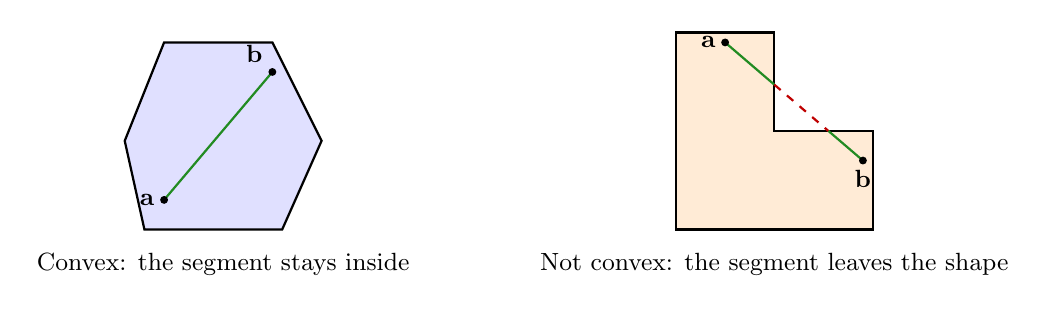
\begin{tikzpicture}[scale=1.25,>=stealth]
\begin{scope}
  \fill[blue!12] (0.2,0) -- (1.6,0) -- (2,0.9) -- (1.5,1.9) -- (0.4,1.9) -- (0,0.9) -- cycle;
  \draw[thick] (0.2,0) -- (1.6,0) -- (2,0.9) -- (1.5,1.9) -- (0.4,1.9) -- (0,0.9) -- cycle;
  \draw[ForestGreen,thick] (0.4,0.3) -- (1.5,1.6);
  \fill (0.4,0.3) circle (0.04) node[left] {\small $\vect{a}$};
  \fill (1.5,1.6) circle (0.04) node[above left] {\small $\vect{b}$};
  \node at (1,-0.35) {\small Convex: the segment stays inside};
\end{scope}
\begin{scope}[xshift=5.6cm]
  \fill[orange!16] (0,0) -- (2,0) -- (2,1) -- (1,1) -- (1,2) -- (0,2) -- cycle;
  \draw[thick] (0,0) -- (2,0) -- (2,1) -- (1,1) -- (1,2) -- (0,2) -- cycle;
  \draw[ForestGreen,thick] (0.5,1.9) -- (1,1.471);
  \draw[red!75!black,thick,dashed] (1,1.471) -- (1.55,1);
  \draw[ForestGreen,thick] (1.55,1) -- (1.9,0.7);
  \fill (0.5,1.9) circle (0.04) node[left] {\small $\vect{a}$};
  \fill (1.9,0.7) circle (0.04) node[below] {\small $\vect{b}$};
  \node at (1,-0.35) {\small Not convex: the segment leaves the shape};
\end{scope}
\end{tikzpicture}
\end{center}

\begin{examplebox}
The L above is the square $[0,2]^2$ with the corner where $x>1$ and $y>1$ removed. Take $\vect{a}=(0.5,\,1.9)$ and
$\vect{b}=(1.9,\,0.7)$, both in the L. Their midpoint is $(1.2,\,1.3)$, which has $x>1$ and $y>1$, so it is in the
removed corner. One point of the segment is outside, so the L is not convex.
\end{examplebox}

\begin{whybox}
\textbf{A half-plane is convex.} If $\vect{n}\cdot\vect{a}\le c$ and $\vect{n}\cdot\vect{b}\le c$, then
$\vect{n}\cdot\big((1-t)\vect{a}+t\vect{b}\big)=(1-t)\,\vect{n}\cdot\vect{a}+t\,\vect{n}\cdot\vect{b}\le(1-t)c+tc=c$.

\textbf{The overlap of convex sets is convex.} If $\vect{a},\vect{b}$ are in every one of the sets, then each set
contains the segment, so the overlap contains it too.

So a convex polygon clipped by half-planes stays convex. That is exactly how a Voronoi cell is built.
\end{whybox}

\textbf{What convexity gives us.}
\begin{itemize}[leftmargin=*]
\item \textbf{Clipping works.} One straight cut of a convex polygon leaves one convex piece, so the walk of
Section~\ref{sec:polygons} returns a single polygon.
\item \textbf{The triangle fan works.} From one vertex, every other vertex is visible, so the fan
$(\vect{v}_0,\vect{v}_k,\vect{v}_{k+1})$ covers the cell with no overlap.
\item \textbf{The centroid is inside the cell.} It is an average of points of the cell, so a Lloyd spot never leaves
the shape.
\item \textbf{Straight flights are safe.} A drone flying straight between two points of a convex cell stays in that
cell, which the safety chain in Part~III relies on.
\end{itemize}

\subsection{What affine means}
An \textbf{affine map} is a matrix followed by a shift:
\[
f(\vect{q})=\vect{c}+\vect{D}\,\vect{q}.
\]
The matrix $\vect{D}$ can scale, squish, rotate or shear, and the vector $\vect{c}$ moves the result. For the DVS,
$\vect{c}=\pW$ and $\vect{D}=\tfrac{r}{r_0}\,\mathrm{diag}(\alpha,\,1/\alpha)$. In code, with $r_0=1$ and one point per
row, this is \texttt{P\_w + r * points @ A.T}.

Everything useful about affine maps comes from one property: \textbf{they keep weighted averages whose weights add up
to 1}.
\begin{equation}
f\big((1-t)\vect{a}+t\vect{b}\big)=(1-t)\,f(\vect{a})+t\,f(\vect{b}).\tag{$\ast$}\label{eq:affavg}
\end{equation}
\begin{whybox}
Write $\vect{c}=(1-t)\vect{c}+t\vect{c}$. Then
$\vect{c}+\vect{D}\big((1-t)\vect{a}+t\vect{b}\big)=(1-t)(\vect{c}+\vect{D}\vect{a})+t(\vect{c}+\vect{D}\vect{b})$.
The weights must add up to 1 for the shift to come out right.
\end{whybox}

\begin{center}
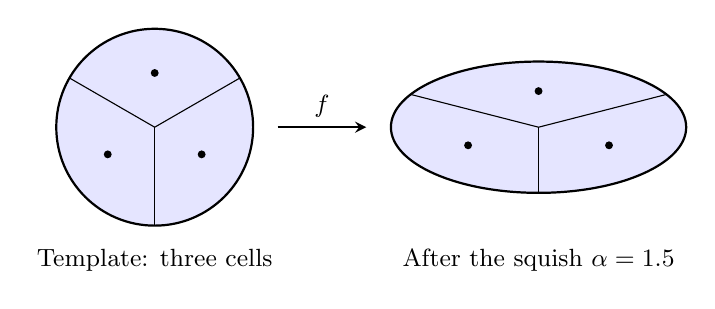
\begin{tikzpicture}[scale=1.25]
\begin{scope}
  \fill[blue!10] (0,0) circle (1);
  \draw[thick] (0,0) circle (1);
  \draw (0,0) -- (0.866,0.5);
  \draw (0,0) -- (-0.866,0.5);
  \draw (0,0) -- (0,-1);
  \fill (0,0.551) circle (0.04);
  \fill (-0.477,-0.276) circle (0.04);
  \fill (0.477,-0.276) circle (0.04);
  \node at (0,-1.35) {\small Template: three cells};
\end{scope}
\draw[->,>=stealth,thick] (1.25,0) -- (2.15,0) node[midway,above] {\small $f$};
\begin{scope}[xshift=3.9cm]
  \fill[blue!10] (0,0) ellipse (1.5 and 0.667);
  \draw[thick] (0,0) ellipse (1.5 and 0.667);
  \draw (0,0) -- (1.299,0.333);
  \draw (0,0) -- (-1.299,0.333);
  \draw (0,0) -- (0,-0.667);
  \fill (0,0.367) circle (0.04);
  \fill (-0.716,-0.184) circle (0.04);
  \fill (0.716,-0.184) circle (0.04);
  \node at (0,-1.35) {\small After the squish $\alpha=1.5$};
\end{scope}
\end{tikzpicture}\\
\small The circle becomes an ellipse. The edges stay straight, the three cells still fill the shape, each cell keeps
the same neighbours, and each spot is still the centroid of its cell.
\end{center}

\begin{center}\small
\begin{tabular}{@{}p{7.4cm}p{7.4cm}@{}}
\toprule
\textbf{Kept by an affine map (with $\det\vect{D}\ne0$)} & \textbf{Not kept}\\
\midrule
Straight lines stay straight & Lengths (Fact~2 gives the bounds)\\
Midpoints, and ratios along a line & Angles: a right angle can stop being right\\
Parallel lines stay parallel & Circles: they become ellipses\\
Convex shapes stay convex & ``Which point is nearest'' (see below)\\
Centroids map to centroids & \\
Which cells touch which & \\
Ratios of areas (all multiplied by $|\det\vect{D}|$) & \\
\bottomrule
\end{tabular}
\end{center}

\begin{whybox}
\textbf{Convex stays convex.} Take two points $f(\vect{x}),f(\vect{y})$ of the image. By ($\ast$), a point on
the segment between them is $f\big((1-t)\vect{x}+t\vect{y}\big)$. Since $X$ is convex, $(1-t)\vect{x}+t\vect{y}$ is in
$X$, so that point is in the image.

\textbf{Centroids map to centroids.} A centroid is an average of the points of a cell, weighted by area, with weights
adding up to 1. Fact~1 multiplies every small area by the same number, so the weights do not change, and
($\ast$) carries the average across.

\textbf{Neighbours stay neighbours.} With $\det\vect{D}\ne0$ the map can be undone, so different points stay different.
Cells cannot start to overlap or leave gaps, and a shared edge maps to a shared edge.
\end{whybox}

\begin{examplebox}
Take $\alpha=2$, $r/r_0=0.5$, so $\vect{D}=\mathrm{diag}(1,\,0.25)$, and $\vect{c}=(3,\,1)$.
\begin{itemize}[leftmargin=*]
\item $\vect{P}=(0,0)\mapsto(3,\,1)$ and $\vect{Q}=(4,2)\mapsto(7,\,1.5)$.
\item Midpoint: $(2,1)\mapsto(5,\,1.25)$, which is exactly the midpoint of $(3,1)$ and $(7,1.5)$.
\item Centroid: the triangle $(0,0),(4,0),(0,4)$ has centroid $(\tfrac43,\tfrac43)\mapsto(\tfrac{13}{3},\tfrac43)$, the
mean of its three mapped corners.
\item Lengths are not kept: the vector $(1,0)$ keeps length $1$, but $(0,1)$ shrinks to $0.25$.
\item Angles are not kept: $(1,1)$ and $(1,-1)$ are perpendicular (dot product $0$). Their images $(1,\,0.25)$ and
$(1,\,-0.25)$ have dot product $0.9375$.
\end{itemize}
\end{examplebox}

\begin{watchbox}
An affine map does \emph{not} keep ``which spot is nearest''. Take spots $\vect{A}=(0,0)$, $\vect{B}=(2,2)$, the point
$\vect{x}=(1.6,\,0)$ and $\vect{D}=\mathrm{diag}(1,\,0.25)$. Before the map, $\vect{x}$ is $1.60$ from $\vect{A}$ and
$2.04$ from $\vect{B}$, so $\vect{A}$ is nearest. After it, the distances are $1.60$ and $0.64$, so $\vect{B}$ is
nearest. So a squished cell is generally \emph{not} the Voronoi cell of the squished spots. That is fine for the DVS:
ownership is decided once on the template and then carried along by the map.
\end{watchbox}

\begin{plainbox}
Put together: Lloyd builds convex cells on the template, once. Moving, scaling and squishing are affine, so during
flight the cells stay convex, still fill the body, keep the same neighbours, and each spot stays the centroid of its
cell. That is why nothing has to be recomputed while flying.
\end{plainbox}

\begin{testbox}
After \texttt{update} with any squish: the centroid of each world cell must equal its world spot
(\texttt{np.allclose}), every cell area must be multiplied by $r^2$ (with $r_0=1$, since the squish has determinant 1), and the
number of vertices of each cell must not change.
\end{testbox}

%------------------------------------------------------------------------------------------
\section{Voronoi cells and the Delaunay graph}\label{sec:voronoi}

Given spots (or drones) $\vect{p}_1,\dots,\vect{p}_n$ inside a region $D$, the \textbf{Voronoi cell} of spot $i$ is
the set of points of $D$ that are at least as close to $\vect{p}_i$ as to any other spot:
\[
V_i=\{\vect{q}\in D:\ \|\vect{q}-\vect{p}_i\|\le\|\vect{q}-\vect{p}_j\|\ \ \forall j\ne i\}.
\]
Each condition ``closer to $i$ than to $j$'' is a \textbf{half-plane}. Expanding the squares,
\[
\|\vect{q}-\vect{p}_i\|^2\le\|\vect{q}-\vect{p}_j\|^2
\iff 2\,\vect{q}\cdot(\vect{p}_j-\vect{p}_i)\le\|\vect{p}_j\|^2-\|\vect{p}_i\|^2
\iff (\vect{q}-\vect{m}_{ij})\cdot\vect{n}_{ij}\le0,
\]
with the midpoint $\vect{m}_{ij}=\tfrac12(\vect{p}_i+\vect{p}_j)$ and the unit normal
$\vect{n}_{ij}=(\vect{p}_j-\vect{p}_i)/\|\vect{p}_j-\vect{p}_i\|$ (the $\|\vect{q}\|^2$ terms cancel, that is why it is
linear). The border between the two half-planes is the perpendicular bisector of $\vect{p}_i\vect{p}_j$.

So $V_i$ is $D$ clipped by $n-1$ half-planes: \textbf{if $D$ is convex, every cell is a convex polygon}, and you can
compute it with the clipping step from Section~\ref{sec:polygons}. Cells do not overlap (except on borders) and
together they cover $D$.

\textbf{Labels on edges.} When you clip cell $i$ by the bisector with $j$ and that bisector survives as an edge of the
final cell, label the edge with the pair $(i,j)$. Edges that come from the border of $D$ get the label $(i,-1)$. These
integer labels are the key to Part III.

\textbf{Delaunay graph.} Connect $i$ and $j$ if their cells share an edge of positive length. This graph is the
``who is my neighbour'' structure of the formation. (For points in general position it is the Delaunay
triangulation; we only need the graph.)

\begin{oursbox}
For tens of drones, simply compute every cell by clipping $D$ with all $n-1$ bisectors: $\mathcal{O}(n^2)$ clips,
microseconds to milliseconds in Python. If $D$ is not convex (a heart, a union of cells after a split), either
clip against its convex hull and then intersect with $D$ by sampling, or use the sampling version of Lloyd
(Section~\ref{sec:lloyd}). \texttt{scipy.spatial.Voronoi} gives the same cells and the pair labels
(\texttt{ridge\_points}) once scipy is installed.
\end{oursbox}

%------------------------------------------------------------------------------------------
\section{Optimisation in five ideas}\label{sec:opt}

\begin{enumerate}
\item \textbf{Gradient.} For a cost $J(\vect{x})$, the gradient $\nabla J$ points uphill; a minimum has $\nabla J=0$.
\item \textbf{Gradient descent.} $\vect{x}\leftarrow\vect{x}-\eta\nabla J(\vect{x})$ with a small step $\eta$.
Simple, but slow when the cost is a long narrow valley.
\item \textbf{L-BFGS.} A quasi-Newton method: it builds an approximation of the curvature (Hessian) from the last few
gradient differences $\nabla J(\vect{x}_{k+1})-\nabla J(\vect{x}_k)$ and uses it to take much better steps. You only
supply $J$ and $\nabla J$. In Python: \texttt{scipy.optimize.minimize(method="L-BFGS-B")}.
\item \textbf{Penalty method.} A constraint $g(\vect{x})\le0$ becomes an extra cost $w\,\max(g(\vect{x}),0)^3$: zero
when the constraint holds, growing when it is violated. The cube makes it smooth (twice differentiable) at $g=0$, so
L-BFGS behaves well. Large $w$ = strict.
\item \textbf{Assignment problem.} Given a cost matrix $C_{ij}$ (cost of giving spot $j$ to drone $i$), find the
one-to-one matching with the smallest total cost. The \textbf{Hungarian algorithm} solves it exactly in
$\mathcal{O}(n^3)$. In Python: \texttt{scipy.optimize.linear\_sum\_assignment(C)}. For $n\le8$, trying all $n!$
permutations is fine for testing.
\end{enumerate}

%==========================================================================================
\part{The paper's DVS, piece by piece}
%==========================================================================================

\section{The big picture}

The swarm does not plan each drone directly. It plans one imaginary body, the \textbf{Deformable Virtual Structure},
that can \emph{move}, \emph{scale} and \emph{squish}. Each drone owns a spot inside the body and follows it. The
pipeline (both the DVS planner and the drones replan at 5\,Hz):
\begin{enumerate}
\item \textbf{PAAS} (PArtitioning and ASsignment): spread $n$ spots evenly over the template shape (Lloyd), and
give each drone a spot (Hungarian). Run again whenever drones join or leave.
\item \textbf{DVS path search}: score a library of short candidate paths, each with a fixed scale and squish, and
pick the best.
\item \textbf{DVS trajectory optimisation}: turn the chosen path into a smooth motion of the body over time,
including how scale and squish change, respecting speed and acceleration limits.
\item \textbf{Per-drone planning}: each drone plans its own path that follows its moving spot and avoids obstacles
and other drones.
\end{enumerate}
The whole state of the body is
\[
\bm\sigma(t)=[\,\pW(t)\T,\ r(t),\ \alpha(t)\,]\T
\qquad(\text{3D: }\R^5;\ \text{our 2D: }[x,y,r,\alpha]\in\R^4),
\]
the centre, the scale and the squish. Every drone target follows from these few numbers, which is why the method
scales to 100 drones.

%------------------------------------------------------------------------------------------
\section{Spreading the spots: coverage and the Lloyd algorithm}\label{sec:lloyd}

\subsection{What is being minimised}
Template shape $W$ (a polygon; for us a circle of radius $r_0$ to start). We want $n$ spots $\vect{p}_{1,c},\dots,
\vect{p}_{n,c}$ (relative to the DVS centre) such that \emph{every point of the shape is close to some spot}. The
standard way to say this:
\begin{equation}
J(\vect{p}_{1,c},\dots,\vect{p}_{n,c})=\sum_{i=1}^{n}\int_{V_i}\|\vect{q}-\vect{p}_{i,c}\|^2\,\rho(\vect{q})\,d\vect{q},
\tag{1, clean form}
\end{equation}
where $V_i$ are the Voronoi cells inside $W$ and $\rho\ge0$ is a density (use $\rho=1$: every part of the shape
equally important).

\begin{watchbox}
The paper prints eq.~(1) as $\int_W\|\vect{q}-\vect{p}_c\|\rho\,d\vect{q}$, with no cells, no square and $\vect{p}_c$
meaning ``the set of spots''. Read it as the clean form above: that is the problem Lloyd's algorithm actually solves.
\end{watchbox}

\subsection{Why the best spot is the centroid of its cell}
Fix the cells for a moment and look at one spot $\vect{p}$ with cell $V$. Write $M=\int_V\rho$ (the cell's mass) and
$\vect{c}=\frac1M\int_V\vect{q}\rho$ (its centroid). Then
\begin{equation}
\int_V\|\vect{q}-\vect{p}\|^2\rho\,d\vect{q}\;=\;\int_V\|\vect{q}-\vect{c}\|^2\rho\,d\vect{q}\;+\;M\,\|\vect{p}-\vect{c}\|^2 .
\label{eq:parallel}
\end{equation}
\begin{whybox}
Write $\vect{q}-\vect{p}=(\vect{q}-\vect{c})+(\vect{c}-\vect{p})$ and expand the square. The cross term is
$2(\vect{c}-\vect{p})\cdot\int_V(\vect{q}-\vect{c})\rho\,d\vect{q}$, and
$\int_V(\vect{q}-\vect{c})\rho=M\vect{c}-M\vect{c}=\vect{0}$ by the definition of the centroid. (This is the
``parallel-axis theorem'' from mechanics.)
\end{whybox}
The first term does not depend on $\vect{p}$, the second is smallest (zero) at $\vect{p}=\vect{c}$. So \textbf{for
fixed cells, each spot should sit at the centroid of its cell}. Equivalently, the gradient is
$\partial J/\partial\vect{p}_{i,c}=2M_i(\vect{p}_{i,c}-\vect{c}_i)$.

\subsection{The algorithm and why it always improves}
\begin{algbox}[Lloyd's algorithm]
\begin{enumerate}[leftmargin=*]
\item Start from seeds (the paper uses a rectangular grid of seeds; any spread-out start works).
\item \textbf{Assign:} compute the Voronoi cells $V_i$ of the current spots inside $W$.
\item \textbf{Move:} replace every spot by the centroid $\vect{c}_i$ of its cell.
\item Repeat 2--3 until the largest move is below a tolerance (e.g.\ $10^{-4}r_0$).
\end{enumerate}
\end{algbox}
Neither step can increase $J$. The \emph{move} step makes the second term of (\ref{eq:parallel}) zero for every cell.
The \emph{assign} step gives every point $\vect{q}$ to its nearest spot, which can only lower
$\|\vect{q}-\vect{p}\|^2$ for that point. $J\ge0$ and decreases every round, so the spots settle. The result is a
\textbf{centroidal Voronoi tessellation}: an even spread that fills odd shapes well.

\begin{center}
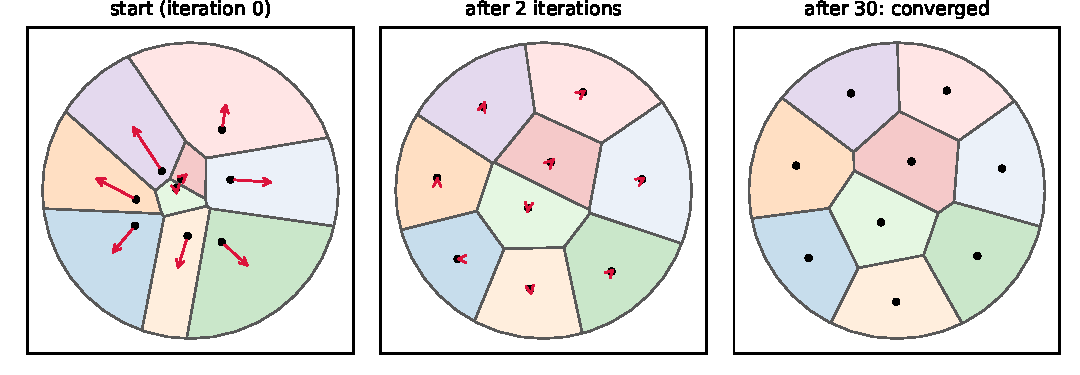
\includegraphics[width=\textwidth]{fig_lloyd.pdf}\\
\small Lloyd on a disk with 9 spots. Red arrows: each spot jumps to the centroid of its cell.
\end{center}

\begin{watchbox}
Lloyd finds a \emph{local} optimum. Perfectly symmetric starts (an exact square grid) can be balance points that it
never leaves, even when a better arrangement exists. A tiny random perturbation of the seeds fixes this (we saw the
same effect in the Voronoi animation).
\end{watchbox}

\begin{oursbox}
Two ways to compute the cells. (a) Exact: clip the disk polygon by bisectors (Section~\ref{sec:voronoi}) and use the
polygon centroid formula. (b) Sampling: cover the shape with a fine grid of sample points, label each by its nearest
spot, and replace each spot by the mean of its samples. (b) works for any shape, even non-convex ones; (a) is exact.
\end{oursbox}

\begin{testbox}
$n=1$: the spot goes to the centre of the disk. $n=2$: the two spots end on a diameter at distance $\tfrac{4r_0}{3\pi}
\approx0.42r_0$ from the centre (the centroid of a half disk). $n=7$: one in the middle, six around. The cost $J$ must
decrease every iteration; print it.
\end{testbox}

\subsection{What Lloyd is for, and how the code does it}

\begin{plainbox}
Lloyd answers one question: \emph{where do I put $n$ spots so that they spread evenly over the shape?} You do not
design a layout by hand. Three drones, seven drones, twenty-three drones: you call the same function with a different
$n$ and get an even arrangement. This is the ``number-adaptive'' part of the paper: if a drone joins or dies, rerun
Lloyd with the new $n$. The result also gives the safety number $l_{\min}$, the closest pair of spots, which sets how
big the body must be (Section~\ref{sec:affine}).
\end{plainbox}

\textbf{Why the spots spread out.} There is no force between them. A spot with a close neighbour on one side has its
cell cut short on that side, while the cell still reaches far on the open side. So the centroid of the cell lies
toward the open space, and moving the spot there takes it away from the crowd. Each spot only ever looks at its own
cell, yet the whole set evens out.

\begin{center}
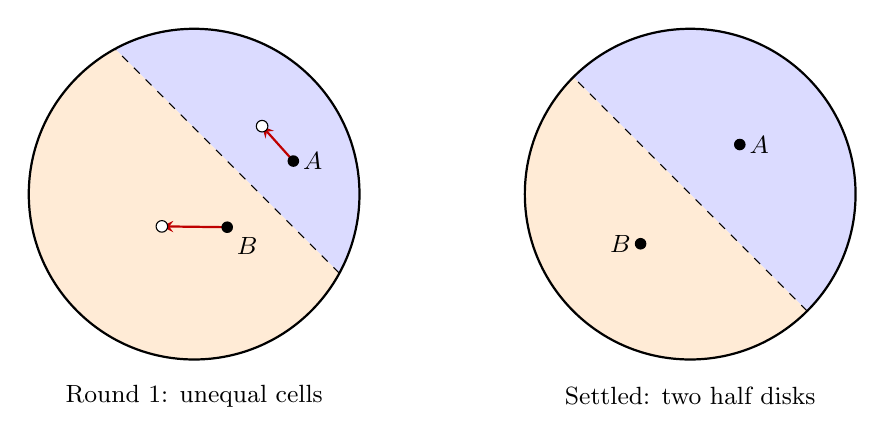
\begin{tikzpicture}[scale=2.1,>=stealth]
\begin{scope}
  \begin{scope}
    \clip (0,0) circle (1);
    \fill[blue!14] (-2,2.4) -- (2.4,-2) -- (3,3) -- cycle;
    \fill[orange!16] (-2,2.4) -- (2.4,-2) -- (-3,-3) -- cycle;
  \end{scope}
  \draw[thick] (0,0) circle (1);
  \draw[dashed] (0.878,-0.478) -- (-0.478,0.878);
  \draw[->,red!75!black,thick] (0.6,0.2) -- (0.411,0.411);
  \draw[->,red!75!black,thick] (0.2,-0.2) -- (-0.195,-0.195);
  \fill (0.6,0.2) circle (0.035) node[right] {\small $A$};
  \fill (0.2,-0.2) circle (0.035) node[below right] {\small $B$};
  \draw[fill=white] (0.411,0.411) circle (0.035);
  \draw[fill=white] (-0.195,-0.195) circle (0.035);
  \node at (0,-1.22) {\small Round 1: unequal cells};
\end{scope}
\begin{scope}[xshift=3cm]
  \begin{scope}
    \clip (0,0) circle (1);
    \fill[blue!14] (-2,2) -- (2,-2) -- (3,3) -- cycle;
    \fill[orange!16] (-2,2) -- (2,-2) -- (-3,-3) -- cycle;
  \end{scope}
  \draw[thick] (0,0) circle (1);
  \draw[dashed] (0.707,-0.707) -- (-0.707,0.707);
  \fill (0.3,0.3) circle (0.035) node[right] {\small $A$};
  \fill (-0.3,-0.3) circle (0.035) node[left] {\small $B$};
  \node at (0,-1.22) {\small Settled: two half disks};
\end{scope}
\end{tikzpicture}\\
\small Dashed: the bisector between the spots. Black dots: spots. White dots: centroids of their cells. Red arrows:
the move made in one round. When settled, each spot is on its own centroid, so nothing moves.
\end{center}

\begin{examplebox}
Unit disk, two spots starting at $A=(0.6,\,0.2)$ and $B=(0.2,\,-0.2)$. These numbers come from running the code:
\begin{center}\small
\begin{tabular}{@{}cccc@{}}
\toprule
Round & $A$ & $B$ & Largest coordinate change\\
\midrule
start & $(0.600,\ 0.200)$ & $(0.200,\ -0.200)$ & --\\
1 & $(0.411,\ 0.411)$ & $(-0.195,\ -0.195)$ & $0.395$\\
2 & $(0.359,\ 0.359)$ & $(-0.243,\ -0.243)$ & $0.052$\\
3 & $(0.332,\ 0.332)$ & $(-0.269,\ -0.269)$ & $0.027$\\
4 & $(0.317,\ 0.317)$ & $(-0.283,\ -0.283)$ & $0.015$\\
20 & $(0.300,\ 0.300)$ & $(-0.300,\ -0.300)$ & below $10^{-6}$\\
\bottomrule
\end{tabular}
\end{center}
Both spots end at distance $\sqrt{0.3^2+0.3^2}=0.424$ from the centre, the half-disk value $\tfrac{4}{3\pi}$. Any
diameter would do equally well; the start decides which one you get.
\end{examplebox}

\textbf{Who moves during Lloyd.} Imaginary points, not drones. The ground station runs every round in milliseconds,
on the fixed template circle at the origin, and only then hands out the final spots. Each spot then rides along with
the body through eq.~(4), so the spread stays with the formation as it moves and scales (a squish stretches it, which
is what the safety scaling in Section~\ref{sec:affine} is for). Lloyd runs again only when the number of drones
changes, not at every control step.

\begin{watchbox}
Do not build the cells from the real drone positions inside the moving world boundary. That is a different method
(coverage control, where the robots themselves are the Lloyd points), and it causes two problems here.
\begin{itemize}[leftmargin=*]
\item If the body moves away faster than a drone can follow, the drone can end up outside the boundary with an
\emph{empty} cell, and the centroid is undefined.
\item The assignment becomes pointless. Each centroid $\vect{c}_i$ lies in the cell of drone $i$, so drone $i$ is the
closest drone to it. The matching ``keep everyone'' is then always the cheapest, and Hungarian has nothing to decide.
\end{itemize}
\end{watchbox}

\begin{oursbox}
The method \texttt{DVS.lloyd} in our code:
{\small
\begin{verbatim}
def lloyd(self, n, iters=500, tol=1e-6):
    rng = np.random.default_rng(0)
    radius = 0.8*np.sqrt(rng.uniform(size=n))
    angle = rng.uniform(0, 2*np.pi, n)
    p_c = np.column_stack([radius*np.cos(angle), radius*np.sin(angle)])

    for _ in range(iters):
        new = np.array([self.centroid(cell)
                        for cell in self.create_cells(p_c)])
        moved = np.abs(new - p_c).max()
        p_c = new
        if moved < tol: break

    return p_c
\end{verbatim}
}
\begin{itemize}[leftmargin=*]
\item \textbf{Start:} $n$ random points in the disk. The square root makes them uniform over the \emph{area}; without
it they bunch up near the centre. The factor $0.8$ keeps them off the edge. A fixed seed gives the same result every
run, and random seeds avoid the symmetric balance points mentioned above.
\item \textbf{Loop:} \texttt{create\_cells} is the assign step, and taking each \texttt{centroid} is the move step.
\item \textbf{Stop:} when no coordinate of any spot changes by more than \texttt{tol}. \texttt{iters} is only a limit
in case convergence is slow.
\end{itemize}
\texttt{update\_drone\_vector} calls this once and then runs the assignment. \texttt{update} runs every step and only
maps the finished spots and cells into the world.
\end{oursbox}

%------------------------------------------------------------------------------------------
\section{Who goes where: the assignment}\label{sec:hung}

After Lloyd we have $n$ spots and $n$ drones. The paper picks the matching $v$ that minimises the total squared travel
(eq.~2):
\begin{equation}
v=\arg\min_{v}\sum_{i=1}^n\big\|\vect{p}_{v(i),c}^{\,\mathrm{world}}-\vect{p}_i\big\|^2 ,\tag{2}
\end{equation}
where $\vect{p}_i$ is where drone $i$ is now, and $\vect{p}^{\,\mathrm{world}}_{j,c}$ is spot $j$ placed in the world
by eq.~(4) below. Build the cost matrix $C_{ij}=\|\vect{s}_j-\vect{p}_i\|^2$ and solve the assignment problem.

\begin{examplebox}
Drones at $x=0,\ 4,\ 10$; spots at $x=1,\ 5,\ 9$ (all on a line). Brute force over the $3!=6$ matchings:
$(1,5,9)$ costs $1+1+1=3$; $(5,1,9)$ costs $25+9+1=35$; $(9,5,1)$ costs $81+1+81=163$; the others are worse than
3. The answer is ``keep the order'', as expected.
\end{examplebox}

\begin{plainbox}
Why squared distances? They punish one long trip much more than several short ones, so the assignment prefers
everybody moving a little. It also tends to avoid crossing paths: if two paths cross, swapping the two targets
always lowers the sum of squares.
\end{plainbox}

%------------------------------------------------------------------------------------------
\section{The body: squish, scale, move}\label{sec:affine}

\subsection{The squish matrix (eq.~3)}
\begin{equation}
\vect{A}=\begin{bmatrix}\alpha_x&0&0\\0&\alpha_y&0\\0&0&1\end{bmatrix},\qquad\alpha_x\alpha_y=1
\quad\Rightarrow\quad \vect{A}_{2D}=\mathrm{diag}(\alpha,\,1/\alpha). \tag{3}
\end{equation}
$z$ is never squished (vertical squish would push drones into each other's downwash). By Fact~1,
$\det\vect{A}_{2D}=\alpha\cdot\frac1\alpha=1$, so \textbf{the squish keeps the area}: a circle of radius $r_0$ becomes
an ellipse with half-axes $\alpha r_0$ and $r_0/\alpha$, area $\pi r_0^2$.

\subsection{Where each drone should be (eq.~4)}
The paper writes $\vect{p}_i=\pW+\vect{p}_{i,c}\cdot\vect{A}\cdot\vect{R}/\vect{R}_0$ with row vectors and an
element-wise division. Because everything is diagonal, the clean column-vector form is
\begin{equation}
\boxed{\ \vect{p}_i(t)=\pW(t)+\vect{S}(t)\,\vect{A}(t)\,\vect{p}_{i,c},\qquad
\vect{S}=\mathrm{diag}\!\big(\tfrac{r}{r_0},\tfrac{r}{r_0},1\big)\ }\tag{4}
\end{equation}
Read it right to left: take the template spot, squish it, scale it, move it to the centre. In 2D,
$\vect{D}=\vect{S}\vect{A}=\mathrm{diag}\big(\tfrac{r}{r_0}\alpha,\ \tfrac{r}{r_0}\tfrac1\alpha\big)$.

\begin{center}
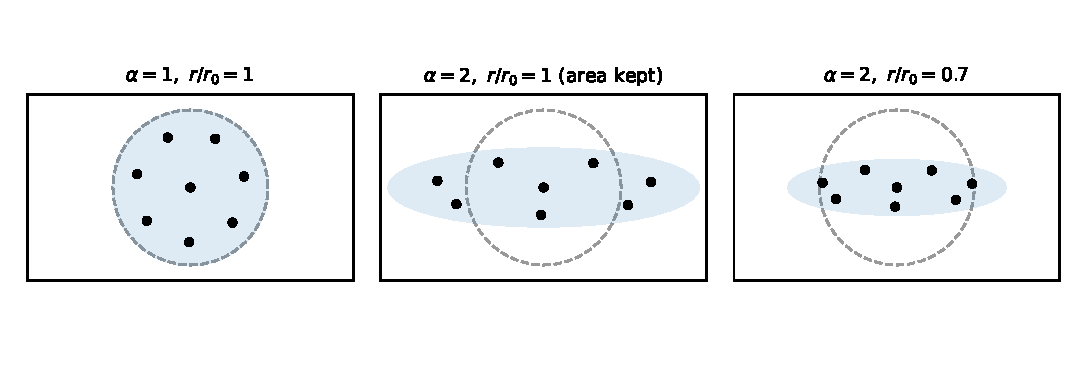
\includegraphics[width=\textwidth]{fig_affine.pdf}\\
\small Middle: the squish keeps the area. Right: the scale changes it. Grey dashed: template circle.
\end{center}

\begin{examplebox}
$\vect{p}_{i,c}=(1,\,0.5)$, $\alpha=2$, $r/r_0=0.8$, $\pW=(10,0)$. Squish: $(2,\,0.25)$. Scale: $(1.6,\,0.2)$. Move:
$\vect{p}_i=(11.6,\,0.2)$.
\end{examplebox}

\subsection{Safety scaling (eq.~5), and the fix for the squish}
Let $l_{\min}=\min_{i\ne j}\|\vect{p}_{i,c}-\vect{p}_{j,c}\|$ (closest template spots) and $l_s=2hr_a$ (the safe
distance: $r_a$ drone radius, $h\ge1$ safety factor). The paper sets
\begin{equation}
r=r_0\,\frac{l_s}{l_{\min}} .\tag{5}
\end{equation}
With $\alpha=1$ the closest pair is then exactly $\tfrac{r}{r_0}l_{\min}=l_s$ apart.

\begin{watchbox}
With a squish this is no longer true. By Fact~2, two spots at template distance $l$ end up at a distance of at least
$\frac{r}{r_0}\min(\alpha,\tfrac1\alpha)\,l$. With $\alpha=2$ the closest pair can shrink to half of $l_s$. To keep the
guarantee for every squish up to $\alpha_{\max}$ (and its inverse), use
\begin{gather*}
r\ \ge\ r_0\,\frac{l_s\,\max(\alpha,1/\alpha)}{l_{\min}}\qquad\text{(at the current }\alpha\text{), or}\\
r=r_0\,\frac{l_s\,\alpha_{\max}}{l_{\min}}\qquad\text{(once, valid for all }\alpha\in[1/\alpha_{\max},\alpha_{\max}]).
\end{gather*}
The paper relies on the drones' own collision avoidance to absorb the difference. In Part III we make it exact.
\end{watchbox}

\begin{examplebox}
$r_a=0.04$\,m (whoop), $h=2$ $\Rightarrow l_s=0.16$\,m. Lloyd gives $l_{\min}=0.35$ for $r_0=1$. Paper: $r=0.457$.
With squishes up to $\alpha_{\max}=1.5$: $r=0.686$, i.e.\ a 50\,\% bigger formation, because the squished direction
needs the room.
\end{examplebox}

%------------------------------------------------------------------------------------------
\section{Choosing a route: primitive path search (eqs.~6--7)}\label{sec:search}

The planner keeps a \textbf{library} of short candidate paths for the body's centre (straight and curved, in several
directions). Each candidate is tried with a few fixed values of $r$ and $\alpha$ (constant along the candidate, for
speed). Every candidate gets a score
\begin{equation}
S=\frac{1}{w_r c_r+w_\alpha c_\alpha+w_o c_o+w_e c_e},\tag{6}
\end{equation}
and the highest score wins. Each cost answers one question:
\begin{itemize}
\item $c_r=(r-r_0)^2$: ``did we resize without need?''
\item $c_\alpha=(\alpha-\alpha_0)^2$: ``did we squish without need?'' ($\alpha_0$ usually 1).
\item $c_o$: ``how much of the body is inside obstacles at the end of the path?'' (eq.~7, below).
\item $c_e$: ``does the path point towards the goal?''
\end{itemize}

\textbf{The obstacle term (eq.~7)} is \emph{the fraction of the (squished, scaled) body that overlaps obstacles}.
Never compute the printed integral; sample it:
\[
c_o\approx\frac1K\sum_{k=1}^K O\big(\vect{p}_p+\vect{D}\,\vect{u}_k\big),\qquad
O(\vect{q})=\begin{cases}1&\vect{q}\text{ in an obstacle}\\0&\text{free}\end{cases}
\]
where $\vect{u}_k$ are $K$ points spread uniformly over the template disk of radius $r_0$ and $\vect{p}_p$ is the
candidate's end point. $c_o=0$: completely free; $c_o=1$: completely blocked.

\begin{watchbox}
Eq.~(7) as printed uses $r$ both as the radius and as the integration variable, has no area element, and its
$(p_x,p_y,p_z)$ is not a proper ball parametrisation. Read it as ``average occupancy over the squished ball'', which
is exactly what the sampling formula computes. To sample a disk uniformly, use radius $r_0\sqrt{U}$ (not $r_0U$) and
angle $2\pi U'$ with $U,U'$ uniform in $[0,1]$; otherwise points crowd at the centre.
\end{watchbox}

\textbf{The direction term} is the cosine between ``towards the final goal'' and ``towards the end of this candidate'':
\[
c_e=\frac{(\vect{p}_{end}-\vect{p}_{now})\cdot(\vect{p}_p-\vect{p}_{now})}{\|\vect{p}_{end}-\vect{p}_{now}\|\,\|\vect{p}_p-\vect{p}_{now}\|}\in[-1,1].
\]
\begin{watchbox}
As printed, a path aimed straight at the goal ($c_e=1$) \emph{increases} the denominator and \emph{lowers} the score:
the sign is wrong. Use the cost $1-c_e$ (0 when aligned, 2 when opposite).
\end{watchbox}

\begin{examplebox}
Weights $w_r=1,\ w_\alpha=1,\ w_o=20,\ w_e=1$, $r_0=1$, a 1.2\,m gap ahead.
Candidate A: straight, $r=1$, $\alpha=1$: the disk hits the walls, $c_o=0.25$, aligned ($1-c_e=0$). Denominator
$0+0+5+0=5$, $S=0.20$.
Candidate B: straight, $r=1$, $\alpha=1.8$ (long and thin): free, $c_o=0$, $c_\alpha=0.64$. Denominator $0.64$,
$S=1.56$.
Candidate C: veers $30^\circ$ away, round, free: $1-c_e=1-\cos30^\circ=0.13$, but it does not lead through the gap.
Denominator $0.134$, $S=7.5$. C wins this one step! This shows why the weights matter and why the paper adds the
goal term: with $w_e$ much larger (say 20), C's denominator is $2.7$, $S=0.37$, and B wins. Tune the weights on simple
scenes first.
\end{examplebox}

%------------------------------------------------------------------------------------------
\section{A smooth motion: the DVS trajectory (eqs.~8--16)}\label{sec:traj}

\subsection{Why polynomials of degree five}
Take one coordinate $x(t)$ that must go from a start state (position, velocity, acceleration) to an end state in
time $T$, as smoothly as possible. ``Smooth'' is measured by the \textbf{jerk} $\dddot x$ (the rate of change of
acceleration, which for a drone is closely related to how fast it must tilt):
\[
\min_{x(\cdot)}\ \int_0^T\dddot x(t)^2\,dt .
\]
\begin{whybox}
Calculus of variations: perturb the optimum, $x+\epsilon\eta$, with $\eta$ and its first two derivatives zero at both
ends (the boundary states are fixed). The cost changes by $2\epsilon\int\dddot x\,\dddot\eta\,dt+O(\epsilon^2)$. Integrate
by parts three times (boundary terms vanish): $-2\epsilon\int x^{(6)}\eta\,dt$. For this to be zero for every $\eta$
we need $x^{(6)}(t)=0$: the optimum is a \textbf{polynomial of degree 5} (quintic).
\end{whybox}
A quintic $x(t)=c_0+c_1t+\dots+c_5t^5$ has 6 coefficients, and there are exactly 6 boundary conditions (3 at each
end), so it is unique. The first three come straight from the start: $c_0=x_0$, $c_1=v_0$, $c_2=a_0/2$. The other
three solve a $3\times3$ system:
\[
\begin{bmatrix}T^3&T^4&T^5\\3T^2&4T^3&5T^4\\6T&12T^2&20T^3\end{bmatrix}
\begin{bmatrix}c_3\\c_4\\c_5\end{bmatrix}=
\begin{bmatrix}x_f-x_0-v_0T-\tfrac12a_0T^2\\ v_f-v_0-a_0T\\ a_f-a_0\end{bmatrix}.
\]
\begin{examplebox}
From rest at 0 to rest at $\Delta=3$\,m in $T=2$\,s. The solution is the famous rest-to-rest profile
\[
x(t)=\Delta\big(10\tau^3-15\tau^4+6\tau^5\big),\qquad\tau=t/T,
\]
so $c_3=10\Delta/T^3=3.75$, $c_4=-15\Delta/T^4=-2.8125$, $c_5=6\Delta/T^5=0.5625$. Peak speed $1.875\,\Delta/T=2.81$\,m/s
(at $t=T/2$), peak acceleration $\frac{10}{\sqrt3}\Delta/T^2=4.33\,\mathrm{m/s^2}$. If $v_{\max}=2$\,m/s this is too
fast: you need $T\ge1.875\cdot3/2=2.81$\,s.
\end{examplebox}
\begin{center}
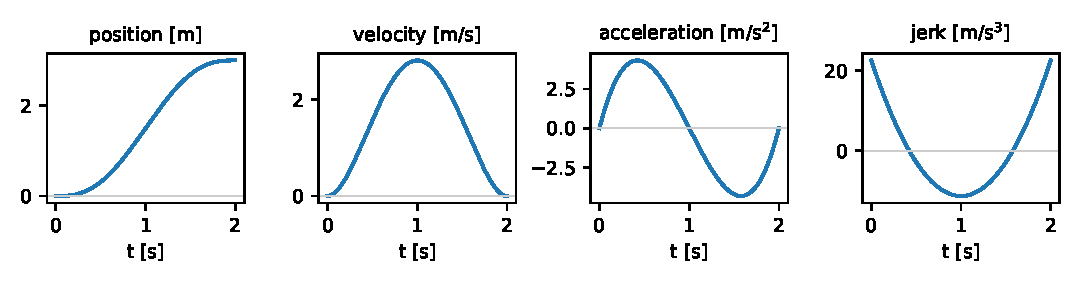
\includegraphics[width=\textwidth]{fig_minjerk.pdf}\\
\small The rest-to-rest minimum-jerk segment of the example.
\end{center}

\subsection{Many pieces glued together (eqs.~8--9) and MINCO}
A long manoeuvre uses $M$ quintic pieces with durations $T_1,\dots,T_M$ and intermediate waypoints
$\vect{q}_1,\dots,\vect{q}_{M-1}$ (for the whole state $\bm\sigma$, so each piece has $6\times m$ coefficients):
\[
\bm\sigma(t)=\vect{c}_i\T\bm\beta(t-t_{i-1})\ \ \text{for }t\in[t_{i-1},t_i),\qquad\bm\beta(t)=[1,t,\dots,t^5]\T.
\tag{8--9}
\]
\textbf{Counting equations.} Per coordinate there are $6M$ unknowns. Conditions: 3 at the start, 3 at the end, and at
each of the $M-1$ inner waypoints: the left piece ends at $\vect{q}_i$, the right piece starts at $\vect{q}_i$, and
derivatives 1 to 4 match (4 more): 6 per waypoint. Total $6+6(M-1)=6M$. So \textbf{waypoints and durations determine
the minimum-jerk trajectory uniquely}, through one (banded, fast) linear system. That map
$(\vect{q},\vect{T})\mapsto\vect{c}$ is what the paper calls \textbf{MINCO}. The optimiser therefore only moves a few
waypoints and durations instead of all coefficients, and continuity (eq.~13) holds automatically.

\subsection{The cost and the constraints (eqs.~10--14)}
\begin{equation}
J=\int_0^{T_\Sigma}\Big(\|\dddot{\vect{p}}_W\|^2+\dddot r^{\,2}+\dddot\alpha^{\,2}\Big)dt+w_T\,T_\Sigma ,\tag{10}
\end{equation}
subject to the start and end states (11), speed and acceleration limits on the body (12), and continuity (13).

\begin{plainbox}
Why the time term $w_TT_\Sigma$? Slowing a trajectory down by a factor $k$ (every duration times $k$) divides the jerk
by $k^3$, so the jerk integral shrinks by $k^5$. Without a price on time the optimiser would make the flight
infinitely slow. $w_T$ sets the trade-off: large $w_T$ flies fast, small $w_T$ flies gently.
\end{plainbox}

\subsection{Why it is enough to check the surface (eqs.~12, 15--16)}
Constraint (12) limits speed and acceleration of sample points $\vect{p}_{j,s}$ on the \emph{outer boundary} of the
body (eq.~16: a grid of points on the template circle/sphere, moved like eq.~4 by eq.~15). Why do the drones inside
not need checking?
\begin{whybox}
A point that sits at template position $\vect{u}$ is at $\vect{x}(t)=\pW(t)+\vect{D}(t)\vect{u}$. Its velocity
$\dot{\vect{x}}=\dot{\vect{p}}_W+\dot{\vect{D}}\vect{u}$ and acceleration $\ddot{\vect{x}}=\ddot{\vect{p}}_W+
\ddot{\vect{D}}\vect{u}$ are \emph{affine} functions of $\vect{u}$. The squared length of an affine function is a
convex function of $\vect{u}$, and a convex function on a disk takes its maximum on the boundary circle (any inside
point is an average of boundary points, and a convex function of an average is at most the average of the values).
So if every boundary point respects $v_{\max}$ and $a_{\max}$, so does every inside point, and every drone.
\end{whybox}
\begin{watchbox}
Eq.~(16) prints the last component as $r\sin(\theta/N_\theta)$; it should be $r\sin(a\theta/N_\theta)$. In 2D the
surface points are simply $N_f$ points $r_0(\cos\phi_j,\sin\phi_j)$, $\phi_j=2\pi j/N_f$.
\end{watchbox}

\subsection{Solving it}
Inequality (12) becomes penalties $w\sum_{\text{samples}}\max(\|\dot{\vect{x}}\|^2-v_{\max}^2,0)^3$ (same for
acceleration), evaluated at a few time samples per piece and at every surface point. Everything is then a smooth
unconstrained cost of $(\vect{q},\vect{T})$, minimised with L-BFGS. Durations must stay positive: optimise
$\tau_i=\log T_i$ instead of $T_i$.

\begin{oursbox}
Start simpler: fix the durations, optimise only the waypoints of a spline through the path-search result, with the
penalties. Add duration optimisation and full MINCO later.
\end{oursbox}

%------------------------------------------------------------------------------------------
\section{Each drone follows its spot (eqs.~17--22)}\label{sec:agent}

Each drone plans its own minimum-jerk path with penalties for dynamics ($\mathcal{J}_d$), obstacles ($\mathcal{J}_o$,
from a distance map), other drones ($\mathcal{J}_s$) and the formation ($\mathcal{J}_f$):
\begin{equation}
\mathcal{J}_f=\sum_{j=0}^{M_c}\|\vect{p}(j)-\vect{p}_{i,f}(j)\|^2 ,\tag{22}
\end{equation}
where $\vect{p}_{i,f}(j)$ is the drone's spot (eq.~4 along the DVS trajectory) at future time stamp $j$. The formation
is a \emph{soft} goal: a drone may leave its spot briefly to avoid something.

\begin{oursbox}
First version: point-mass drones with a tracking controller plus repulsion,
\[
\vect{a}_i=k_p(\vect{p}_{i,f}-\vect{p}_i)+k_d(\dot{\vect{p}}_{i,f}-\dot{\vect{p}}_i)+\sum_{\text{nearby}}
k_{rep}\Big(\frac1d-\frac1{d_0}\Big)\frac{\vect{e}}{d^2},
\]
clipped to $\|\vect{a}_i\|\le a_{\max}$, where $d<d_0$ is the distance to a neighbour or obstacle and $\vect{e}$ the
unit vector pointing away from it. Choose $k_d\approx2\sqrt{k_p}$ (critically damped).
\end{oursbox}

%------------------------------------------------------------------------------------------
\section{The paper's numbers (our targets)}
\begin{center}\small
\begin{tabular}{@{}lccccc@{}}
\toprule
Gap width & 3.2\,m & 2.8\,m & 2.4\,m & 2.0\,m & 1.6\,m\\
\midrule
Paper (DG): success / time & 100\,\% / 7.41\,s & 100 / 7.43 & 100 / 7.39 & 100 / 7.42 & 100 / 7.48\\
SF & 100 / 7.99 & 100 / 8.61 & 100 / 8.59 & 100 / 8.30 & 100 / 8.35\\
SF-ALAS & 100 / 7.11 & 94 / 7.15 & 86 / 7.28 & 30 / 7.30 & 26 / 7.33\\
Rigid structure (VRB) & 100 / 7.07 & 0 & 0 & 0 & 0\\
\bottomrule
\end{tabular}
\end{center}
Limits $v_{\max}=2$\,m/s, $a_{\max}=7\,\mathrm{m/s^2}$; start 7\,m before and stop 7\,m after the gap when the formation
error is below 0.05; 50 trials per width; planning at 5\,Hz; PAAS takes about 0.16\,s for 100 drones.

%==========================================================================================
\part{Our extension: cells, splitting, merging, and a safety chain}
%==========================================================================================

The paper's body is always \emph{one} connected shape. It cannot split around a pillar and join again. Here every drone
owns a cell, a DVS is a \emph{set of cells}, and splitting and merging are operations on sets. Everything uses only the
tools of Part I.

\section{The formation as a cell complex}\label{sec:complex}

\textbf{Objects.} The region of a DVS is $D$. The drones' cells $V_1,\dots,V_n$ (Voronoi cells clipped to $D$, Section
\ref{sec:voronoi}) are polygons stored as CCW vertex lists, and every edge carries its pair label $(i,j)$: $j$ is the
neighbour across the edge, or $-1$ for the border of $D$. A \textbf{group} is a set of drone indices $I$; its region is
$D_I=\bigcup_{i\in I}V_i$.

\textbf{The boundary by cancellation.} Give each cell its CCW boundary: a list of directed edges. Add up the boundaries
of all cells in the group. An edge shared by two cells of the group appears twice, \emph{in opposite directions}
(CCW in one cell is clockwise in the other), and the two copies cancel. What remains is exactly the boundary of the
group:
\[
\partial D_I=\sum_{i\in I}\partial V_i\qquad(\text{shared edges cancel}).
\]
This is the boundary operator $\partial$ from Crane's notes (discrete exterior calculus): a group is a \emph{2-chain},
its boundary a \emph{1-chain}, and $\partial\partial=0$ says the boundary is made of closed loops.

\textbf{With pair labels it is pure bookkeeping:}
\begin{center}\small
\begin{tabular}{@{}lll@{}}
\toprule
Edge of cell $i\in I$ with label $(i,j)$ & Meaning & Kept in $\partial D_I$?\\
\midrule
$j\in I$ & inside the group & no (cancels with the copy in cell $j$)\\
$j\notin I$, $j\ge0$ & border with another group & yes (part of a split line)\\
$j=-1$ & border of the region $D$ & yes (outer boundary)\\
\bottomrule
\end{tabular}
\end{center}
Only integers are compared, so the test is exact; never match edges by comparing floating-point coordinates.

\begin{center}
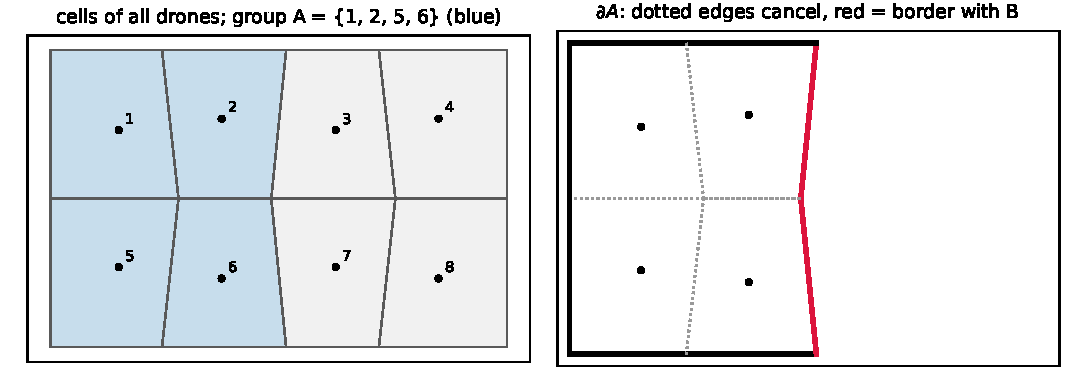
\includegraphics[width=\textwidth]{fig_complex.pdf}\\
\small Left: eight cells, group $A=\{1,2,5,6\}$ in blue. Right: the boundary of $A$. Dotted edges are shared inside $A$
and cancel; black is the outer border; red is the border with the rest.
\end{center}

\begin{watchbox}
Do not maintain cells and edges incrementally. Drones move every step, neighbours change, and edges appear and
disappear. \textbf{Rebuild the cells from scratch at every step} and derive everything (boundaries, neighbours) from the
fresh cells. For tens of drones this is cheap and removes a whole class of bugs.
\end{watchbox}

\begin{testbox}
For any group, the outer boundary edges must chain into closed loops (each vertex used by exactly two boundary edges).
The shoelace area of $\partial D_I$ must equal the sum of the cell areas. For the whole formation ($I$ = all drones)
only edges labelled $-1$ remain.
\end{testbox}

%------------------------------------------------------------------------------------------
\section{Neighbours and cuts: how to split}\label{sec:split}

\textbf{The Delaunay graph} $G$ has the drones as nodes and an edge $(i,j)$ whenever cells $i$ and $j$ share an edge
(read it off the pair labels). A \textbf{split} is a partition of the drones into two groups $I_A\cup I_B$. The edges of
$G$ between the groups are the \textbf{cut}; the \textbf{split line} is the chain of cell borders with labels $(i,j)$,
$i\in I_A$, $j\in I_B$. So we cut along the cell borders, never through a cell.

\textbf{What makes a good split.}
\begin{enumerate}
\item \textbf{Each group connected} in $G$ (check with a breadth-first search), so each part is one piece.
\item \textbf{Each group fits its passage.} A group of $k$ drones needs room for $k$ drones at spacing $l_s$. The
densest possible arrangement is hexagonal, where each drone owns a regular hexagon whose inner radius is $l_s/2$,
with area $\tfrac{\sqrt3}{2}l_s^2$. So a group of $k$ drones needs an area of at least
\begin{equation}
A_{\min}(k)=k\cdot\frac{\sqrt3}{2}\,l_s^2 .
\label{eq:area}
\end{equation}
In practice use $A_{\min}/\eta$ with $\eta\approx0.8$--$0.9$, since Lloyd does not reach a perfect hexagonal packing.
It also needs a minimum width: with $c$ drones side by side, roughly $(c-1)l_s+2(r_a+m)$, where $m$ is the boundary
margin. These two numbers give the \textbf{capacity} of each side of the obstacle, and the sizes $k_A,k_B$ must fit.
\item \textbf{Few cut edges.} A short split line means few drones are disturbed.
\end{enumerate}

\begin{algbox}[Choosing the split by region growing]
\begin{enumerate}[leftmargin=*]
\item Decide $k_A$ from the capacities of the two passages (left and right of the obstacle), $k_B=n-k_A$.
\item Seed group $A$ with the drone nearest to the left passage.
\item Repeatedly add the neighbour (in $G$) of the current group that is nearest to the left passage, until $A$ has
$k_A$ drones. $B$ is the rest.
\item Check that $B$ is connected; if not, try the next seed. For small $n$ you can also brute-force all connected
splits of the right size and keep the one with the fewest cut edges.
\end{enumerate}
\end{algbox}

\begin{center}
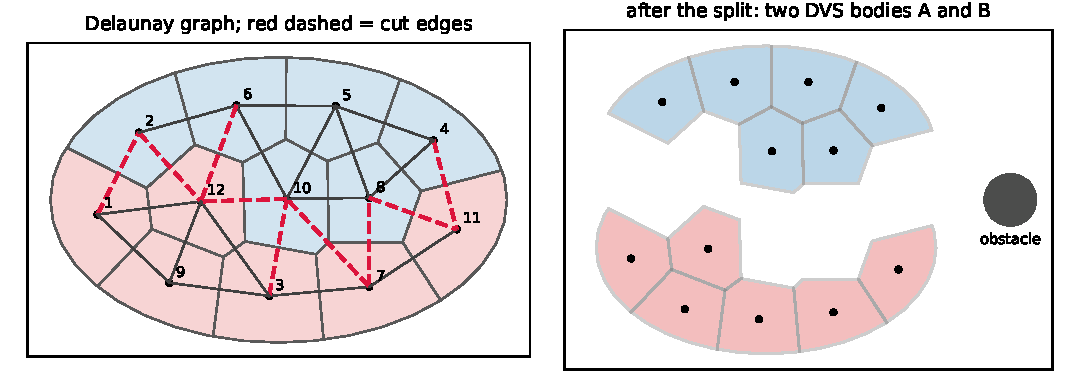
\includegraphics[width=\textwidth]{fig_split.pdf}\\
\small Left: cells and the Delaunay graph; red dashed edges are cut. Right: after the split, two bodies move apart.
\end{center}

\textbf{After the split.} Each group becomes its own DVS with its own state $\bm\sigma_A$, $\bm\sigma_B$ and plans its own
path (path search and trajectory, Sections~\ref{sec:search}--\ref{sec:traj}). Its region starts as the jagged union of
its cells. Relax it to a clean shape over $1$--$2$\,s: a disk (or ellipse) centred at the group's centroid with area at
least $A_{\min}(k)/\eta$. A simple way is a radial blend around the centroid $\vect{c}$:
\[
R_s(\phi)=(1-s)\,R_{\text{union}}(\phi)+s\,R_{\text{disk}},\qquad s:0\to1,
\]
where $R_{\text{union}}(\phi)$ is the distance from $\vect{c}$ to the union's boundary in direction $\phi$. This is valid
when the union is star-shaped around its centroid, which is the normal case for a compact group. Lloyd runs inside the
current blended region while it changes.

\textbf{Fitting the paper's state to a region.} To give a region an equivalent $(\pW,r,\alpha)$, use its centroid
$\vect{c}$ and its covariance $\vect{\Sigma}=\frac1A\int_D(\vect{q}-\vect{c})(\vect{q}-\vect{c})\T d\vect{q}$ with eigenvalues
$\lambda_1\ge\lambda_2$. For an ellipse with half-axes $a,b$ these are $a^2/4$ and $b^2/4$. Since $a=\alpha r$ and
$b=r/\alpha$:
\[
\pW=\vect{c},\qquad \alpha=\Big(\frac{\lambda_1}{\lambda_2}\Big)^{1/4},\qquad r=2\,(\lambda_1\lambda_2)^{1/4},
\]
and the squish axis is the eigenvector of $\lambda_1$.

%------------------------------------------------------------------------------------------
\section{After the cut: reshaping a piece, and splitting into layers}\label{sec:reshape}

\definecolor{spotc}{HTML}{2a78d6}
\definecolor{dronec}{HTML}{eb6834}
\tikzset{piece/.style={draw=gray!70,line width=0.5pt,fill=gray!8},
         target/.style={draw=spotc,dashed,line width=0.6pt},
         path/.style={draw=gray!75,line width=0.45pt},
         start/.style={fill=dronec}, spot/.style={fill=spotc}}

Right after a split, each group's region is the jagged union of its cells. Section~\ref{sec:split} relaxes it to a
clean disk. This section asks \emph{how the spots should travel} during that relaxing, compares three ways, and then
looks at a different kind of split: one body on top of another.

\subsection{What must hold while a piece reshapes}
\begin{enumerate}[leftmargin=*]
\item \textbf{No jumps.} At the split moment every drone's target is where it already was.
\item \textbf{Spacing at every moment.} Any two spots stay at least $l_s$ apart during the whole reshape, not only
at the end.
\item \textbf{Connected neighbours.} If drones rely on neighbours (for example, drones that measure each other
through overlapping floor views), the neighbour graph must stay connected, and ideally change little.
\item \textbf{A good final spread.} At the end, the spots are a Lloyd layout of the new shape.
\end{enumerate}

\subsection{Three ways to move the spots}

\textbf{(a) Interpolate.} Compute the final Lloyd layout $\vect{b}_i$ of the new shape once, seeded from the current
spots $\vect{a}_i$. Match them with the Hungarian method, and move every spot along a straight line,
\[
\vect{s}_i(\tau)=(1-\tau)\,\vect{a}_i+\tau\,\vect{b}_i,\qquad \tau:0\to1,
\]
all starting and ending together. This is the idea of CAPT (Turpin, Michael and Kumar, 2014): with the
sum-of-squares matching, the straight paths cannot cross, and the authors give a spacing condition on start and goal
positions under which the paths are also collision-free. Check their exact condition before relying on it.

\textbf{(b) Lloyd flow.} Blend the region from the piece to the disk (the radial blend of Section~\ref{sec:split}).
At each step, sample the current region, compute each spot's cell centroid $\vect{c}_i$, and move part of the way:
$\vect{s}_i\leftarrow\vect{s}_i+k(\vect{c}_i-\vect{s}_i)$ with $0<k\le1$.

\textbf{(c) SOM flow.} The same as (b), but each spot also listens to its neighbours. Take the neighbour graph of
the spots at the split moment and let $H_{ij}$ be the number of graph steps between $i$ and $j$. With samples
$\vect{x}_n$ of the current region and $b(n)$ the spot nearest to $\vect{x}_n$:
\[
\vect{t}_i=\frac{\sum_n e^{-H_{b(n)i}^2/2\sigma^2}\ \vect{x}_n}{\sum_n e^{-H_{b(n)i}^2/2\sigma^2}},\qquad
\vect{s}_i\leftarrow\vect{s}_i+k(\vect{t}_i-\vect{s}_i).
\]
This is the batch SOM rule with the graph in place of a grid. Shrink $\sigma$ at the end so the layout finishes as a
Lloyd layout.

\begin{whybox}
With $\sigma\to0$ the weight is $1$ for $i=b(n)$ and $0$ otherwise, so $\vect{t}_i$ is the mean of the samples in
cell $i$: exactly the centroid of (b). A SOM flow is a Lloyd flow in which samples won by a neighbour also pull a
little. That pull is what keeps neighbours together, and it is also what pulls spots towards each other.
\end{whybox}

\subsection{A test}
Twenty spots spread by Lloyd over the unit disk are split by the sign of $x$, giving a piece of 9 to 11 spots. The
piece relaxes to a disk of the same area around its centroid over 50 steps, followed by 30 steps of settling.
Four random starts were averaged. ``Closest pair'' is the smallest distance between any two spots at any moment of
the reshape. ``Neighbour changes'' is the largest number of neighbour-graph edges gained or lost compared with the
start. ``Path'' is the mean distance a spot travels.

\begin{center}\small
\begin{tabular}{@{}lcccc@{}}
\toprule
Method & Closest pair (during) & Neighbour changes & Path & Final coverage\\
\midrule
(a) Interpolate & $0.296$ & $6.8$ & $\mathbf{0.199}$ & $0.0269$\\
(b) Lloyd flow & $\mathbf{0.299}$ & $7.8$ & $0.347$ & $0.0269$\\
(c) SOM flow, $\sigma=0.4$ & $0.272$ & $6.0$ & $0.375$ & $0.0271$\\
(c) SOM flow, $\sigma=0.6$ & $0.177$ & $5.0$ & $0.510$ & $0.0279$\\
(c) SOM flow, $\sigma=0.8$ & $0.122$ & $\mathbf{4.5}$ & $0.592$ & $0.0283$\\
\bottomrule
\end{tabular}
\end{center}

\begin{center}
\begin{tikzpicture}[scale=1.45]
\foreach \k/\name/\lab in {0/interp/{(a) Interpolate},1/lloyd/{(b) Lloyd flow},2/som/{(c) SOM flow, $\sigma=0.6$}}{
\begin{scope}[xshift=\k*2.35cm]
  \input{reshape_figs/\name.tex}
  \node at (-0.45,-1.25) {\small \lab};
\end{scope}}
\end{tikzpicture}\\
\small One start. Grey: the piece right after the split. Dashed blue: the target disk. Orange: spots at the split
moment. Blue: where they end. Grey lines: the paths. (a) goes straight; (b) and (c) wander while the region changes,
and (c) first draws the group together before spreading it out again.
\end{center}

\begin{watchbox}
The SOM keeps neighbours together, as hoped: with a wide neighbourhood the neighbour graph changes about a third
less. But it does so by pulling the spots towards each other, and the closest pair during the reshape drops by up to
60\,\%. Spacing is our hard constraint, so in this test the SOM is the wrong trade. It is worth reconsidering only if
an unchanged neighbour graph is itself a hard requirement, and then with a small $\sigma$ and the spacing checked at
every step.
\end{watchbox}

\begin{oursbox}
Use (a): interpolate to a fresh Lloyd layout matched by the Hungarian method. It has the shortest paths, keeps the
spacing as well as the Lloyd flow, ends at the same spread, and comes with the CAPT reasoning for why straight
synchronised paths do not collide. Check the closest pair along the paths anyway: it is a cheap test, done once per
split.
\end{oursbox}

\subsection{Splitting into layers: one body on top of another}
A split does not have to be side by side. Two groups can also fly as two bodies at different heights, one above the
other. In 2D terms each body keeps its own state $(\pW,r,\alpha,\theta)$ and gains a height $z$.

\textbf{What it buys.} A body of $k$ drones needs an area of about $A_{\min}(k)/\eta$ (eq.~\ref{eq:area}). Stacking
$n$ drones as two layers of $n/2$ halves the area each layer needs, so each layer is about $1/\sqrt2\approx0.71$ times
as wide. That helps with a gap that is narrow but tall, such as a door or a window.

\textbf{What it costs.}
\begin{itemize}[leftmargin=*]
\item \textbf{Downwash.} A drone pushes air downwards, and a drone below it loses lift and can be pushed off course.
That is why the paper never squishes in $z$. Treat each drone as needing a horizontal distance $l_s$ \emph{or} a
vertical distance $h_{dw}$ from every other drone, where $h_{dw}$ is the downwash height. Measure $h_{dw}$ for the
whoops; it is much larger than $l_s$.
\item \textbf{Floor cameras.} The upper layer's bottom cameras see the lower drones, which move differently from the
floor. Floor tracking must reject those points. (It could also be turned around: the upper drones could detect the
lower ones directly, a relative measurement for free.)
\item \textbf{Energy and room.} Climbing costs battery, and the space needs the height.
\end{itemize}

\textbf{The safe order of moves.} The dangerous moment is when a drone is directly above another without enough
height between them. So:
\begin{itemize}[leftmargin=*]
\item \textbf{To stack:} the group that goes up first climbs \emph{beside} the other group, until the height
difference is at least $h_{dw}$. Only then does it slide over.
\item \textbf{To unstack:} the upper group first slides away until every horizontal distance is at least $l_s$, and
only then descends.
\end{itemize}
In terms of the rule above: at every moment, every pair has horizontal distance $\ge l_s$ or vertical distance
$\ge h_{dw}$. Climbing beside and sliding over keep the first condition while the second is being built, and the
other way round when unstacking.

\begin{plainbox}
The paper already uses layers, but only for a 3D target shape, giving each layer a number of drones in proportion to
its area. Stacking as a \emph{split}, with its own transition rule and downwash constraint, is ours. Keep it as an
option for later: side-by-side splits come first, and stacking needs a measured $h_{dw}$ before it can be planned
safely.
\end{plainbox}

\begin{testbox}
For each reshape method, record the closest pair at every step, not just at the end. For a stacking transition,
check at every step that each pair satisfies ``horizontal $\ge l_s$ or vertical $\ge h_{dw}$''; a single step where
both fail is a bug.
\end{testbox}

%------------------------------------------------------------------------------------------
\section{Merging: hysteresis, touching, filling, shrinking}\label{sec:merge}

\textbf{When are two groups allowed to merge? (hysteresis).} Right after a split the two groups touch along the split
line, so ``merge when touching'' alone would undo the split at once. Rule:
\begin{algbox}[Merge rule for a pair of groups $A,B$]
Let $d_{AB}(t)$ be the smallest distance between their boundaries (minimum of segment-to-segment distances,
Section~\ref{sec:polygons}).
\begin{enumerate}[leftmargin=*]
\item After a split, set \texttt{separated = False}.
\item When $d_{AB}>d_{sep}$ (for example $d_{sep}=l_s$), set \texttt{separated = True}: they have really moved apart.
\item Merge when \texttt{separated} \textbf{and} $d_{AB}\le\epsilon$ \textbf{and} $\dot d_{AB}<0$ (approaching) \textbf{and}
the filling region $G$ (below) is obstacle-free.
\end{enumerate}
\end{algbox}
\begin{plainbox}
``Apart, then back.'' A pillar between the groups makes them separate by at least its width plus two margins, so they
cannot touch \emph{through} the pillar. They touch only once both have passed it.
\end{plainbox}

\textbf{Filling the waist.} Two round bodies that just touch form a figure eight with a narrow waist, a bad shape for a
formation. Replace $A\cup B$ by its \textbf{convex hull} (the shape a rubber band around both would take; compute it
with the monotone-chain algorithm on the boundary vertices). The added part is $G=\operatorname{hull}(A\cup B)
\setminus(A\cup B)$, and the new region is
\[
D'=A\cup B\cup G=\operatorname{hull}(A\cup B).
\]
Check that $G$ is obstacle-free (sample it like $c_o$). If not, wait and keep the two bodies as they are.

\begin{center}
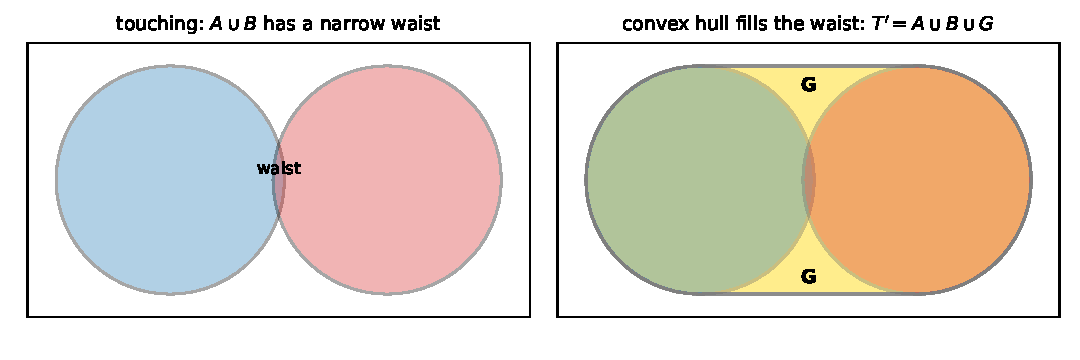
\includegraphics[width=\textwidth]{fig_merge.pdf}\\
\small Left: touching bodies with a waist. Right: the hull adds the yellow regions $G$.
\end{center}

\textbf{Healing and shrinking.} In $D'$ the drones next to $G$ suddenly own very large cells, so Lloyd pulls them into
$G$ and the formation becomes solid. Then shrink the target region smoothly from the hull to the nominal shape (a
disk), with the radial blend above. The final area must not go below the area rule (\ref{eq:area}) with all $n$
drones: $A_{\text{final}}\ge n\frac{\sqrt3}{2}l_s^2/\eta$. Finally fit $(\pW,r,\alpha)$ to the merged region and continue
as one DVS.

%------------------------------------------------------------------------------------------
\section{The safety chain}\label{sec:safety}

We want: no drone ever touches another drone or an obstacle. Three links, each simple to check.

\textbf{Link (a), drone--drone: buffered cells.} The buffered cell of drone $i$ is its cell shrunk by $l_s/2$ from every
bisector:
\[
B_i=\{\vect{q}\in V_i:\ (\vect{q}-\vect{m}_{ij})\cdot\vect{n}_{ij}\le-\tfrac{l_s}{2}\ \ \forall j\ne i\}.
\]
\textbf{Claim:} if every drone stays inside its own buffered cell, every pair stays at least $l_s$ apart.
\begin{whybox}
For a pair $i,j$: $\vect{p}_i\in B_i$ gives $(\vect{p}_i-\vect{m}_{ij})\cdot\vect{n}_{ij}\le-\tfrac{l_s}2$. For drone $j$
the normal is reversed, $\vect{n}_{ji}=-\vect{n}_{ij}$ (same midpoint), so $\vect{p}_j\in B_j$ gives
$(\vect{p}_j-\vect{m}_{ij})\cdot\vect{n}_{ij}\ge\tfrac{l_s}2$. Subtract: $(\vect{p}_j-\vect{p}_i)\cdot\vect{n}_{ij}\ge l_s$.
Since $\vect{n}_{ij}$ is a unit vector, $\|\vect{p}_j-\vect{p}_i\|\ge l_s$.
\textbf{During motion:} compute the $B_i$ at the start of a step and move each drone in a straight line inside its own
$B_i$. A convex set contains the segment between any two of its points, so at every moment of the step each drone is in
its own $B_i$, and the separation holds continuously, not only at the samples.
\end{whybox}
\begin{center}
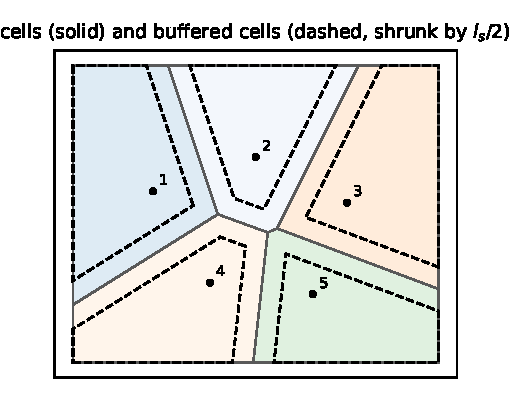
\includegraphics[width=0.55\textwidth]{fig_buffered.pdf}
\end{center}

\textbf{Link (b), drone--boundary: the body never shrinks onto a drone.} Require for every drone of a group
\[
d\big(\vect{p}_i,\partial D_I\big)\ \ge\ r_a+m_b
\]
(point-to-polygon distance, Section~\ref{sec:polygons}; $m_b$ a small margin). Then the whole disk of the drone lies inside
the region.

\textbf{Link (c), boundary--obstacles.} The region keeps a margin from obstacles: $D_I$ does not overlap the obstacles
inflated by $m_o$. In the path score this means $c_o=0$ for the inflated map (stricter than the paper, which tolerates a
little overlap).

\textbf{Putting them together.} (b) puts each drone's disk inside its group's region, (c) keeps the region off obstacles,
so no drone touches an obstacle. (a) keeps drones apart inside a group. Between groups, the separate regions plus
the margins keep them apart, and they only come together through the merge rule.

\textbf{What (b) means for the planner: a limit on shrinking speed.} If the region shrinks faster than the drones can
move inward, (b) would break. Over one planning step $\Delta t$ a drone can move at most about $v_{\max}\Delta t$. So the
inward speed of the boundary must stay below what the drones can follow:
\[
-\,\vect{n}_{out}\cdot\dot{\vect{p}}_{j,s}\ \le\ u_{\max}<v_{\max}\qquad\text{for every surface point }j,
\]
where $\vect{n}_{out}$ is the outward normal of the boundary at that point. Add it to the DVS trajectory optimisation as
one more penalty, like eq.~(12). If the path search wants a faster squeeze, the optimiser slows the manoeuvre down
instead.

\begin{watchbox}
All three links concern the \emph{estimated} positions. With optical-flow drift the true positions differ by up to the
drift $e(t)$. To stay honest, increase every margin by the drift bound: $l_s\to l_s+2e(t)$, $m_b\to m_b+e(t)$,
$m_o\to m_o+e(t)$, with $e(t)$ growing with flight time.
\end{watchbox}

\textbf{Height.} All bodies fly at one height $z_{DVS}$; drone $i$ may have an offset $h_i$ along the vertical, so
$z_i=z_{DVS}+h_i$. Offsets help spacing only if they clear the downwash: two drones closer than $l_s$ horizontally need
$|h_i-h_j|\ge z_{dw}$. Keep offsets either equal or at least $z_{dw}$ apart.

%------------------------------------------------------------------------------------------
\section{Build order and checks}
\begin{center}\small
\begin{tabular}{@{}p{0.4cm}p{5.3cm}p{8.6cm}@{}}
\toprule
\# & Piece & Done when\\
\midrule
1 & Polygon tools (area, centroid, inside, distances, clipping) & unit square and triangle examples match by hand\\
2 & Voronoi cells with pair labels & cells cover the disk; areas add up to the disk area\\
3 & Lloyd & $J$ decreases; $n=1,2,7$ tests of Section~\ref{sec:lloyd}\\
4 & Assignment & 3-drone example gives ``keep the order''\\
5 & Body transform, eq.~(4), squish-safe scaling & area constant for any $\alpha$; closest pair $\ge l_s$ for all $\alpha\le\alpha_{\max}$\\
6 & Obstacle map, $c_o$ by sampling & 0 in free space, rises smoothly into walls\\
7 & Path score and library (with $1-c_e$) & thin squished candidate wins in front of a narrow gap\\
8 & Smooth trajectory (spline + penalties) & surface points respect $v_{\max},a_{\max}$\\
9 & Point-mass drones following spots & tracking error small, no collisions\\
10 & Join/leave: rerun 3--5 & formation re-forms, no long crossings\\
11 & Cell complex and boundary by cancellation & tests of Section~\ref{sec:complex}\\
12 & Delaunay graph, connectivity, split by region growing & both groups connected and within capacity\\
13 & Two DVS bodies, relax to clean shapes & each body flies its own path around a pillar\\
14 & Merge rule (apart, then back), hull, healing, shrink & no instant re-merge; merged area $\ge$ area rule\\
15 & Safety chain (a)--(c) and shrink-speed limit & distances never below $l_s$, $r_a+m_b$, $m_o$ in 50 random runs\\
16 & Benchmarks & paper's gap test, plus pillar-in-corridor and two-gap scenes\\
\bottomrule
\end{tabular}
\end{center}

%------------------------------------------------------------------------------------------
\section{Symbol glossary}
\begin{center}\small
\begin{tabular}{@{}>{$}l<{$}p{12.6cm}@{}}
\toprule
n & number of drones\\
W,\ D,\ D_I & template shape; region of a DVS; region of group $I$\\
\vect{p}_{i,c},\ \vect{p}_i & template spot of drone $i$; its position (now or target)\\
V_i,\ B_i & Voronoi cell of drone $i$; its buffered cell (shrunk by $l_s/2$)\\
\vect{m}_{ij},\ \vect{n}_{ij} & midpoint and unit normal of the bisector between $i$ and $j$\\
(i,j),\ (i,-1) & pair label of an edge: neighbour $j$, or border of the region\\
\rho,\ M_i,\ \vect{c}_i & density; mass and centroid of cell $i$\\
\pW,\ r,\ r_0,\ \alpha & body centre, scale, template scale, squish\\
\vect{A},\ \vect{S},\ \vect{D}=\vect{S}\vect{A} & squish matrix, scale matrix, their product\\
l_{\min},\ l_s,\ r_a,\ h & closest template spots; safe distance $2hr_a$; drone radius; safety factor\\
S,\ c_r,\ c_\alpha,\ c_o,\ c_e,\ w_\ast & path score, its costs (use $1-c_e$), weights\\
\bm\sigma,\ M,\ T_i,\ T_\Sigma & body state, number of pieces, piece durations, total time\\
\vect{q}_i,\ \vect{c}_i\ (\text{traj.}) & waypoints; polynomial coefficients of piece $i$\\
v_{\max},\ a_{\max},\ u_{\max} & speed, acceleration, and boundary inward-speed limits\\
\vect{p}_{j,s},\ N_f & surface sample points of the body; their number\\
A_{\min}(k),\ \eta & area rule for $k$ drones; packing efficiency of Lloyd\\
d_{AB},\ d_{sep},\ \epsilon & boundary distance between groups; separation and touch thresholds\\
G,\ D' & filling region of a merge; merged region (convex hull)\\
m_b,\ m_o,\ e(t) & boundary and obstacle margins; drift bound\\
\bottomrule
\end{tabular}
\end{center}

\end{document}
